\documentclass[10pt]{article}
%\documentclass[10pt]{book}

\usepackage[draft]{fixme}
%\usepackage[final]{fixme}

\usepackage{listings}

\usepackage{html}
\usepackage{color}

\usepackage{multicol}
\usepackage{multirow}

\usepackage{graphicx}
\usepackage{alltt}

\usepackage{pdfpages}

\newcommand{\hlstd}[1]{\textcolor[rgb]{0,0,0}{#1}}
\newcommand{\hlkey}[1]{\textcolor[rgb]{0,0,0}{\bf{#1}}}
\newcommand{\hlnum}[1]{\textcolor[rgb]{0.16,0.16,1}{#1}}
\newcommand{\hltyp}[1]{\textcolor[rgb]{0.51,0,0}{#1}}
\newcommand{\hlesc}[1]{\textcolor[rgb]{1,0,1}{#1}}
\newcommand{\hlstr}[1]{\textcolor[rgb]{1,0,0}{#1}}
\newcommand{\hldstr}[1]{\textcolor[rgb]{0.51,0.51,0}{#1}}
\newcommand{\hlcom}[1]{\textcolor[rgb]{0.51,0.51,0.51}{\it{#1}}}
\newcommand{\hldir}[1]{\textcolor[rgb]{0,0.51,0}{#1}}
\newcommand{\hlsym}[1]{\textcolor[rgb]{0,0,0}{#1}}
\newcommand{\hlline}[1]{\textcolor[rgb]{0.33,0.33,0.33}{#1}}

\newcommand{\mySmallFontSize}{\scriptsize}
\newcommand{\mySmallestFontSize}{\tiny}

\newcommand{\codeFontSize}{\scriptsize}
\newcommand{\code}[1]{{\scriptsize #1}}

\newcommand{\SeedingExampleDirectory}{../../../projects/bugSeeding}
\newcommand{\SeedingExampleBuildDirectory}{../..//projects/bugSeeding}

% Software version number
\newcommand{\VersionNumber}{0.9.5a}

\newcommand{\ExampleDirectory}{../../../projects/compass/tests}

% Latex trick to allow us to comment out large sections of documentation
\newcommand{\commentout}[1]{}

% change the title of the Fixme List
\renewcommand{\listfixmename}{Things to Fix in Documentation of Compass}

\newcommand{\comm}[2]{\bigskip
                      \begin{tabular}{|p{11cm}|}\hline
                      \multicolumn{1}{|c|}{{\bf Comment by #1}}\\ \hline
                      #2\\ \hline
                      \end{tabular}
                      \bigskip
                     }

\def\verbatimfile#1{\begingroup
                    \@verbatim \frenchspacing \@vobeyspaces
                    \input#1 \endgroup
}



\newcounter{lineno}

% Taken from verbatimfiles.sty on web
\makeatletter %JCL

\def\verbatimlisting#1{\setcounter{lineno}{0}%
    \begingroup \@verbatim \frenchspacing \@vobeyspaces \parindent=20pt
    \everypar{\stepcounter{lineno}\llap{\thelineno\ \ }}\input#1
    \endgroup
}

\makeatother

% \endinput


%\addtolength{\oddsidemargin}{-0.5in}
%\addtolength{\evensidemargin}{-0.5in}
\addtolength{\textheight}{0.5in}
%\addtolength{\textwidth}{0.5in}
%\addtolength{\textwidth}{1.0in}
%\addtolength{\topmargin}{-0.5in}
%\addtolength{\textheight}{1.5in}

% \pagenumbering{roman}
% \pagestyle{empty}
% \setcounter{page}{0}
% \thispagestyle{empty}

\sloppy

%---------------------------------------------------------------------
% Begin Document
%---------------------------------------------------------------------

\begin{document}

% This draft mode eliminates the figures (leaves boxes for where they would be)
%\psdraft

\title{ {\bf Automated Seeding Of Security Flaws For The Construction Of Test Suites To Evaluate Static Analysis Tools \\
                              \textcolor{blue}{Design Document} \\
                                  \textcolor{red}{ Draft } } }
%\title{ {\bf \textcolor{red}{         Bug Seeding Design: \\
%                       A Tool for the Evaluation of Static Analysis Tools \\
%                                        (A ROSE Tool)} \\
%                       \textcolor{blue}{Draft User Manual} \\
%                       \textcolor{green}{(Associated with ROSE Version 0.9.5a)} } }

% This doesn't seem to work.  References to this label are not resolved.
\label{BugSeeding:postscriptVersionOfUserManual}

\author{Dan Quinlan, others to be defined on basis of collaborations}

\begin{htmlonly}
   \centering \includegraphics[width=3in]{../compass_rose.gif}
\end{htmlonly}

\maketitle

\begin{htmlonly}
   \centering \includegraphics[width=5in]{../compass_rose.gif}
\end{htmlonly}

% \newpage

\chapter{Introduction}

\section{Overview}

\label{introduction::overview}

   Compass is a tool for the checking of source code.  It is
based on the ROSE compiler infrastructure and demonstrates to
use of ROSE to build lots of simple pattern detectors for analysis
of C, C++, and Fortran source code.

   The purpose of this work is several fold:
\begin{itemize}
   \item Provide a concrete tool to support interactions with lab customers.
   \item Provide a home for the security analysis specific detectors being built within
         external research projects.
   \item Provide an external tool for general analysis of software.
   \item Provide a tool to support improvements to the ROSE source code base.
   \item Define an infrastructure for an evolving and easily tailored program analysis tool.
   \item Provide a simple motivation for expanded use of ROSE by external users.
         Development, testing, and evaluation of ROSE infrastructure is best facilitated 
         through its expanded use by others and this provides a specific and attractive
         tool that can provide feedback to users about their own code projects.  Even
         though optimization research is our focus, this gets our supporting
         infrastructure for optimization research out and into use by others in the form
         of an extensible tool.
\end{itemize}

   Note that as the collection of detectors grows we will periodically reorganize the 
collection.  At some point soon we will build a hierarchy to organize the evolving
collection.

%\subsection{A basis for other source analysis tools}
\paragraph{A basis for other source analysis tools}
   Input and output to ROSE is organized so that any number of source could be used.
So although we provide a compiler interface (for simplicity), we will also provide a 
GUI interface as an alternative interface to demonstrate that the detectors are orthogonal
to there use in alternative tools.  Alternative tool interfaces should be possible 
and will further demonstrate the independence of the input and output mechanisms to
the designs and implementation of the core detectors.

\paragraph{Add Your Own Detector}

    Detectors written in Compass make direct use of ROSE and are 
designed to be copied and extended by users to develop their own 
detectors. We welcome the contribution of these detectors back to 
the ROSE team for inclusion into future releases of Compass;
full credit for all work will be provide to all authors.
Compass is an open source project using ROSE, an open source
compiler infrastructure.

    Each of the detectors are examples of how to
add your own detector to {\bf Compass}.  If you
build a detector that you would like to have be 
distributed with {\bf Compass}, please send it to
us and we will add your as an external contributor.

  Guidelines for contributions:
\begin{itemize}
   \item Use any Compass detector and an example.
   \item provide the documentation about your detector.
   \item Use any features in ROSE to support your detector; AST, Control Flow graph,
    System dependence Graph, Call Graph, Class Hierarchy Graph, etc.
   \item Your detector should have {\bf NO} side-effects on the AST.
\end{itemize}






\chapter{Design}


\section{Use Cases}

\label{design::UseCase}

Figure~\ref{Compass_usecase} shows the use cases of \emph{Compass}.
Compass as a tool is used to analyze source code. The analysis is triggered by the user who
selects which detectors to execute. The user also specifies the source code to be checked.
Results of the analysis are presented to that user.

\begin{figure}[th]
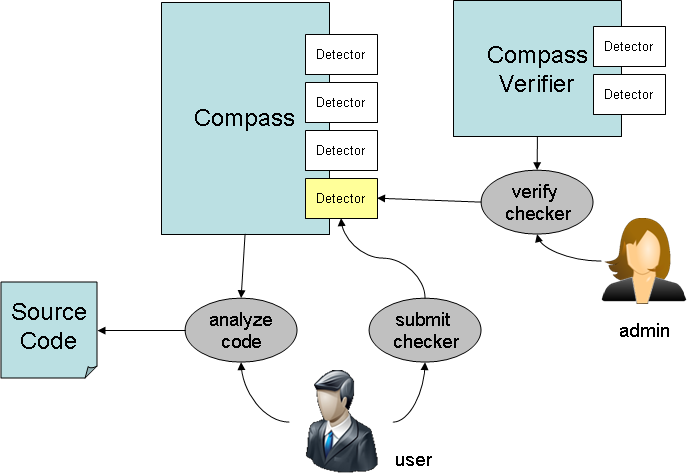
\includegraphics[width=4.5in]{compass_pic.png}
\caption{Compass Use Case}
\label{Compass_usecase}
\end{figure}

Furthermore, a user may contribute with his own detectors that he can add to Compass. Since 
external users may contribute detectors automatically via scripts, a verification of the 
validity and safety of these detectors is necessary. We provide a \emph{Compass Verifier}
that helps to check that all detectors are safe. Currently, the verifier is run by
a administrative person but may run automatically in the future.



\section{Design}

\begin{figure}[thb]
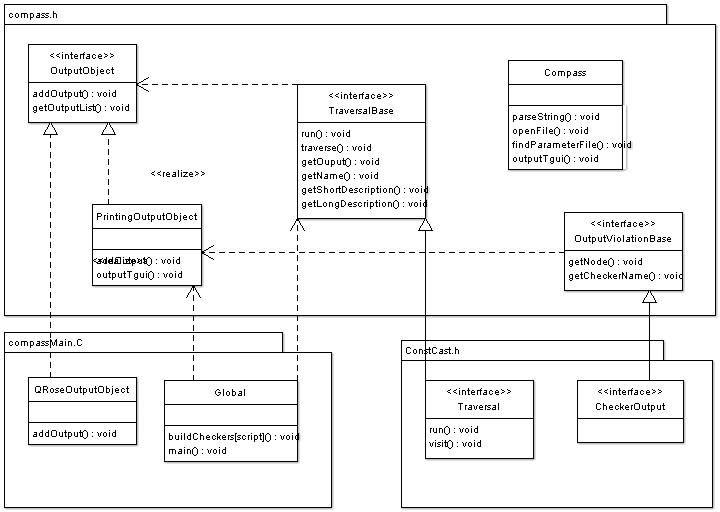
\includegraphics[width=6.0in]{compassdesign.png}
\caption{Compass Design}
\label{CompassDesign}
\end{figure}

Compass is designed to be easy to extend. Any user may write a detector and add it to Compass. Figure~\ref{CompassDesign}
illustrates the UML design decisions behind Compass.


Most of the functionality of Compass is in abstract classes hidden in the Compass namespace within compass.h - a file within
the compassSupport directory. All detectors, such as ConstCast illustrated in the figure, utilize the abstract classes
to traverse a program with all its nodes and to output violations found in that code according to the local algorithm.

CompassMain is the main executable that initially calls ROSE to parse a program. Then \emph{buildCheckers} is called to
load all detectors that are specified within a configuration file. The configuration file allows users to turn on and off
specific detectors for their run-time analyses. However, the configuration file only permits detectors to be loaded that 
were part of Compass at compile-time.

The main interface file compass.h contains the abstract classes \emph{TraversalBase} and 
\emph{OutputObject}. TraversalBase is the interface to ROSE, allowing a detector to traverse the ROSE AST (program) and hence
perform analysis on that AST. OutputObject aids to output defects found by a specific detector. More functionality to handle
e.g. file input and parameters provided to Compass, is provided within the Compass namespace.


\section{Compass Verifier}

\subsection{Threats} 

Compass must be safe, so that analyses and their results can be trusted. 
The main threats to the validity of Compass are:

\begin{itemize}
\item \emph{Malicious User}. A malicious user is an external user of Compass contributing a detector that performs malicious behaviour.  
\item \emph{Malicious Detector}. Compass is extensible and new detectos can be added externally (users outside the main development group).
  A detector can be programmed arbitrarily using the C/C++ and assembly programming languages. 
  It is therefore possible for a skilled programmer to hide malicious operations within a detector, e.g. allow a detector to scan the host machine and
  send data away. Compass must prevent detectors with malicious behaviour to be part of the Compass system. 
\item \emph{Source Code Replacement}. It should not be possible for users to exchange the source code of detectors within a running system,
  i.e. Compass cannot implement dynamic loading of detectors. Such a feature would compromise its safety.
\item \emph{Binary Replacement}. Another threat is the replacement of a valid Compass detector with a modified malicious version within a binary release of Compass.
  Therefore, Compass should be aware if parts of itself were modified and should not execute.
\end{itemize} 

\subsection{Safety Handling}

Compass is designed to be safe. The Compass Verifier is a stable separate copy of Compass that contains only a few detectors
to check (external and internal) user delivered detectors for safety. We have designed Compass in a way that it addresses the threats mentioned above:

\begin{itemize}
\item \emph{Malicious User}. Initially, we permit only trusted individuals to add new detectors to Compass. Once the verification process
  is matured, we will extend this policy to allow arbitrary users to contribute to Compass. 

\item \emph{Malicious Detector}. To prevent Compass to execute malicious code, the Compass Verifier executes its own detectors on
any user defined detector that is beeing considered to be added to Compass.
Currently, the Compass Verifier contains three detectors:

\begin{itemize}
\item \emph{fileReadOnlyAccess} ensures that a user defined detector perorms no write or execute operations on files. 
\item \emph{forbiddenFunctions} is a white list of function calls permitted in a detector. This list contains functions
that are trusted and hence considered unharmful when integrated to Compass.
\item \emph{noAsmStmtsOps} searches for assembly instructions in a detector and flags those as unsafe.
\end{itemize}

\item \emph{Source Code Replacement}. Detectors can only be added at compile time to Compass, not at run-time.
This means that detectors (meaning the source code) cannot be exchanged against unsafe versions at run-time. Furthermore, we allow only 
the Compass tool builder (admin) to build versions of Compass that must pass the Compass Verifier.

\item \emph{Binary Replacement}. Our goal is to perform a MD5 checksum on all the detectors part of the binary Compass distribution before
  Compass is executed. In this way Compass will not run if parts of it were modified.
\end{itemize} 


%The above list contains an important subset of detectors that enforce Compass detectors to be safe. 
%Additional detectors can easily be added to that list.
%In the future, a detector submitted to Compass, should go first through the automatic verifier, before it is either 
%added to Compass or denied.  




\newpage


\chapter{Design and Verification}

Compass is a tool is used to analyze software (both source code and binaries). 
A collection of {\em checkers} are built with each of them detecting the 
violation of a rule.  By reporting on the violations of rules {\em Compass} provides 
a way to enforce predefined or arbitrary user specified properties on software.
This chapter covers the design of {\em Compass} and the design of the verification in 
the \emph{Compass Verifier}, used to verify properties of the checkers implemented 
and submitted to {\em Compass}.

% \section{Use Cases}
\section{Usage Model}

\label{design::UseCase}

Figure~\ref{Compass_usecase} shows the usage model (use cases) of \emph{Compass}.
The analysis is triggered by the user running {\em Compass} over an
input file (source code or binary). The user implicitly selects 
which checkers to execute (defining what rules are to be enforced); 
by default all checkers are run. 
The user also specifies the input file to be checked; for source code 
the specification is similar to the command line required for the 
compilation in the case of a source file.  Results of the analysis 
are presented to the user, a number of mechanisms can be used to 
display the results.

\begin{figure}[th]
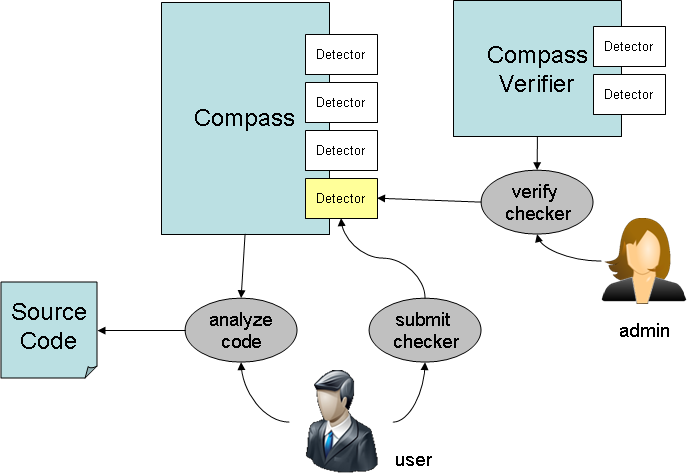
\includegraphics[width=4.5in]{compass_pic.png}
\caption{Compass Use Case}
\label{Compass_usecase}
\end{figure}

Either the same user or a different user/developer can also
implement and submit checkers to be built into Compass.
% Furthermore, a user may contribute with his own checkers that can be added to Compass. 
Since external users may contribute checker automatically via scripts, a verification of the 
validity and safety of these checkers is necessary. We provide a \emph{Compass Verifier}
that helps to check that all checkers are safe. Currently, the verifier is run by
an administrative person but may run automatically in the future.

%\section{Assumption of trust} 
\section{Trust Model}
By design we make a few assumptions about the use of Compass in order to define
a secure tool. We assume:
\begin{enumerate}
   \item For now, there is an assumption of trust in the person writing the checker. \\
      We use the \emph{Compass Verifier} as a way to double check the 
      checkers so that we can eventually weaken the level of trust assumed for people 
      writing checkers. However, the design of the \emph{Compass Verifier} is not likely to
      ever be robust enough to guarantee an automated proof of security for each checker.  
      Thus, we also assume that someone trusted will also review the checker.
      {\em not implemented: We expect that a digital signature (using a key mechanism) 
           is possible to associate a trusted reviewer with a review of 
           the checker together with a strong hash function that
           digitally signs the checker source code.}

   \item Since running \emph{Compass Verifier} is an optional part of building 
      the Compass executable, the person running these test is trusted. There are
      two ways to run the \emph{Compass Verifier} (see section \ref{sec:compass_verify}
    for details):
      \begin{itemize}
         \item Slow: once on each checker ({\tt make verify}). This mechanism
            tests all the files one checker at a time and thus can not miss 
            a file.  Note that even the counter examples are tests which can 
            be a problem when the counter example for the checker is detected
            as a violation for \emph{Compass Verifier}.  Counter examples for
            checkers have to be carefully written to not represent examples that
            violate \emph{Compass Verifier}.
         \item Fast: once on the union of all the checkers ({\tt make oneBigVerify}).
            This step forms a single file of all the checkers (and in-doing so can
            miss some files, and so is less secure).  It is mostly for testing 
            purposes.
      \end{itemize}

   \item The person building the Compass executable is trusted.

   \item The environment where the testing using Compass is done is trusted.

   \item Compass is designed so that the user running Compass need not be trusted.

\end{enumerate}

It is unclear at present how weak the assumption of trust on the compass checker developer 
can be and it may ultimately depend directly on the capabilities of the \emph{Compass Verifier}.


\section{Architecture}

\begin{figure}[thb]
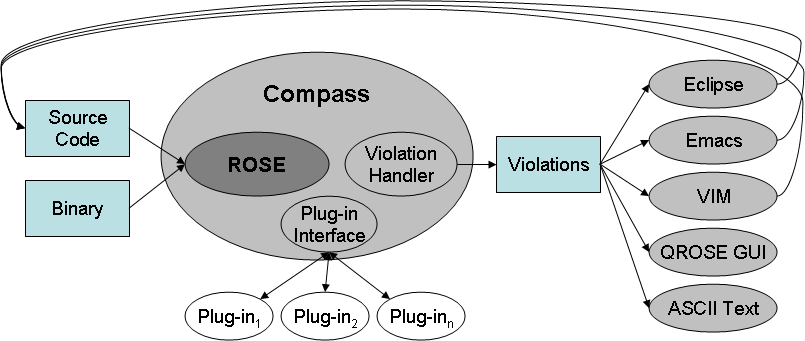
\includegraphics[width=6.0in]{compass_arc.png}
\caption{Compass Architecture}
\label{CompassArchitecture}
\end{figure}


Compass is a tool that allows users to implement checkers to locate and
report software defects.
Documentation of various kinds of software defects can be found in sources
such as the CERT Secure Coding Rules, Common Weakness Enumeration from MITRE, 
and other sources. Our focus is not to define new software defects but
rather to provide a platform that allows the easy implementation of defect
checkers.  Compass has been designed to be easy to extend, allowing users to 
implement their own custom checkers (custom source code analyses for
identifying defects), as shown in Figure~\ref{CompassArchitecture}. Compass supports
the implementation of both simple as well as more advanced defect
checkers. For the latter, Compass utilizes the ROSE infrastructure to
perform a wide range of general purpose program analyses, such as control
flow analysis, data flow analysis, program slicing, etc.


Compass is designed in a way that allows users who do not necessarily have
compiler backgrounds to utilize the ROSE infrastructure to build their
own analysis tools.
Compass is foremost an extensible open source infrastructure for the
development of large
collections of rules. Our current implementation supports automatic
defect checking, programming language restriction, and malware detection in
C, C++, and object code.
Support for Fortran is a new addition to ROSE and will be supported in
Compass in the near future.




\section{Design}

\begin{figure}[thb]
\hspace{-1.5in}
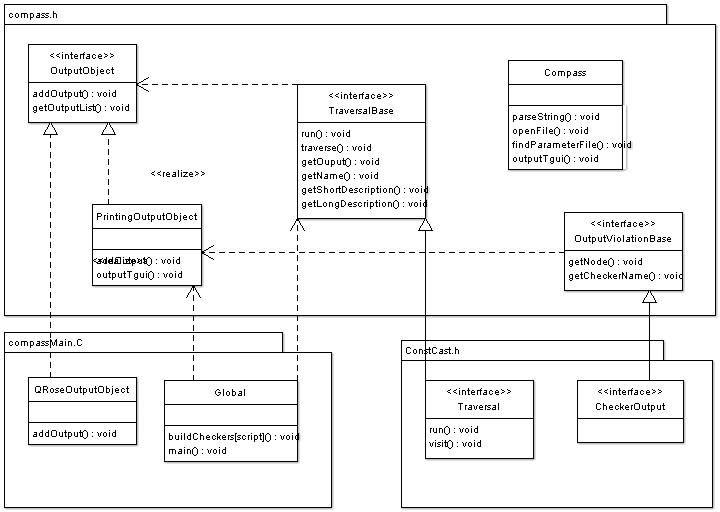
\includegraphics[width=7in]{compassdesign.png}
%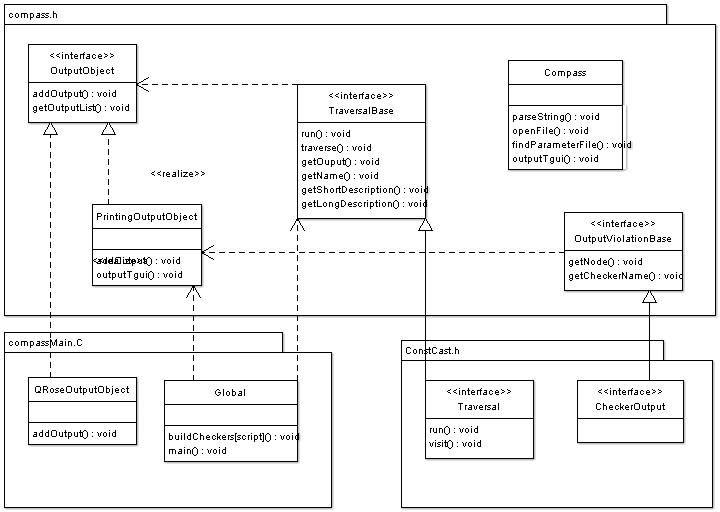
\includegraphics[width=6.0in]{compassdesign.png}
\caption{Compass Design}
\label{CompassDesign}
\end{figure}

Compass is designed to be easy to extend. Any user may write a checker and add it to
Compass. Figure~\ref{CompassDesign} illustrates the UML design decisions behind Compass.


Most of the functionality of Compass is in abstract classes hidden in the Compass
namespace within compass.h - a file within the compassSupport directory. The figure uses a
specific example, {\em ConstCast}, for illustration; Compass is designed to support a large
number of checkers (hundreds). All checkers, such as the {\em ConstCast} checker (illustrated in
figure~\ref{CompassDesign}), utilize the abstract classes to traverse a program with all
its nodes and to output violations found in that code according to the local algorithm.

CompassMain is the main executable that initially calls ROSE to parse a program. Then
\emph{buildCheckers} is called to load all checkers that are specified within a
configuration file. The configuration file allows users to turn on and turn off specific
checkers for their run-time analyses. However, the configuration file only permits
checkers to be loaded that were part of Compass at compile-time.

The main interface file compass.h contains the abstract classes \emph{TraversalBase} and 
\emph{OutputObject}. TraversalBase is the interface to ROSE, allowing a checker to
traverse the ROSE AST (program) and hence perform analysis on that AST. OutputObject aids
to output defects found by a specific checker. More functionality to handle e.g. file
input and parameters provided to Compass, is provided within the Compass namespace.

\section{Compass Verifier}

Compass must be safe, so that analyses and their results can be trusted. 
The {\em Compass Verifier} is used at build time to run a specific set of separate 
compass rules offer the source code of all the checkers.  For simplicity it runs in two
modes: fast, for checking specific named checker source files; and slow, for testing 
{\em all} checker source files.

\subsection{Threats} 

In order to define a complete design for security we outline the threats that
understand to be relevant. The main threats to the validity of Compass checkers are:
\begin{itemize}
\item \emph{Malicious User} \\ 
  A malicious user is an external user of Compass contributing a checker that performs malicious behavior.
\item \emph{Malicious Checker} \\ 
  Compass is extensible and new checkers can be added externally (users outside the main development group).
  A checker can be programmed arbitrarily using the C/C++ and assembly programming languages. 
  It is therefore possible for a skilled programmer to hide malicious operations within a
  checker.  Compass must prevent checkers with malicious behavior to be part of the
  Compass system. Threats are:
   \begin{itemize}
      \item {\bf exfiltration} \\
         A checker should act in a secure way with the input files it is given.
         Securing the inputs to Compass (e.g. the inputs to each checker) from 
         exfiltation is a first priority. Allowing a checker to scan the host 
         machine to exfiltrate arbitrary data (this is a threat that any secure
         software will have).
      \item {\bf modification of filesystem} \\
         A checker should be side-effect free, or have only well defined side-effects, 
         but a malicious checker could modify or erase parts of the accessible file 
         system (e.g. deleting whole directory structures).
%     \item {\bf others ??? ...}
   \end{itemize}

\item \emph{Malicious Compass} \\
    Since Compass is built from ROSE, it is possible to modify compass (or any checker) 
    to generate source code that could be compiled to replace the existing executable
    (there are some constraints here) or regenerate the source code to replace the 
    existing source code or perhaps just provide an alternative copy of the source code.
    This indirect transformation of the input code is a threat.

\item \emph{Source Code Replacement} \\ It should not be possible for users to exchange the
    source code of checkers within a running system, i.e. Compass cannot implement dynamic
    loading of checkers. Such a feature would compromise its safety.

\item \emph{Binary Replacement} \\ Another threat is the replacement of a valid Compass
    checker with a modified malicious version within a binary release of Compass.
    Therefore, Compass should be aware if parts of itself were modified and should not
    execute.

\end{itemize} 

%\subsection{Safety Handling}
\subsection{Mitigation of Threats}

Compass is designed to be safe. The Compass Verifier is a stable separate copy of Compass
that contains only a few checkers to check (external and internal) user delivered checkers
for safety.  We have hopefully designed Compass in a way that it addresses the threats
mentioned above:
\begin{itemize}
\item \emph{Malicious User} \\ Initially, we permit only trusted individuals to add new
    checkers to Compass. Once the verification process is matured, we will extend this
    policy to allow less trusted users to contribute to Compass. A goal will be to allow
    arbitrary users to contribute checkers, however, a review of the whole Compass design
    (and the {\em Compass Verifier} especially) will be required to define required trust
    levels for user/developers who implement checkers.
\fixme{We might define trusted and untrusted checkers as a way to have checkers from
       arbitrary users, but mark them as untrusted.}

\item \emph{Malicious Checker} \\ To prevent Compass from executing malicious code, the Compass
    Verifier executes its own checkers on any user defined checker that is being
    considered to be added to Compass. Currently, the Compass Verifier contains three checkers:
   \begin{itemize}
      \item \emph{fileReadOnlyAccess} ensures that a user defined checker performs no write
         or execute operations on files.
      \item \emph{allowedFunctions} is a {\em white list} of function calls permitted in
         a checker. This list contains functions that are trusted and hence considered
         safe when integrated to Compass.
\fixme{This is not yet implemented as a white list and is instead currently a black list; called: forbiddenFunctions.}
      \item \emph{noAsmStmtsOps} searches for assembly instructions in a checker and flags
         and reports all cases as unsafe.
      \item To avoid modifications of the AST for the purpose of allowing other checkers
         to pass, the AST should not be modified (this should extend to all the
         program analysis graphs generated and used by other checkers).
         {\em This is not implemented yet.} 
\end{itemize}

\item \emph{Malicious Compass} \\
    Since Compass does not generate code, it can not be used to modify the input software
    (source code or binary) or generate a new copy that could be confused with the input.
    However, future versions of Compass make make transformation to introduce greater
    levels of security; fix flaws, mitigate specific forms of threats, etc.  It will be
    important to make sure that such transformation can not change the behavior of an
    input code to make the modified input code malicious.  Current proposed approaches
    would build a patch which would have to be inspected by a trusted developer before
    it would be applied to modify the input code.

\item \emph{Source Code Replacement} \\ Checkers can only be added at compile time to
    Compass, not at run-time. This means that checkers (meaning the source code) cannot be
    exchanged against unsafe versions at run-time. Furthermore, we allow only the Compass
    tool builder (admin) to build versions of Compass that must pass the Compass Verifier.

\item \emph{Binary Replacement} \\ 
    Our goal is to perform a strong hash (e.g. Secure Hash Algorithm - SHA2) as a 
    checksum on all the checkers
    part of the binary Compass distribution before Compass is executed. In this way
    Compass will not run if parts of it were modified. {\em This is not implemented yet.}
\fixme{We should describe the policy for allowing SHA2 to be verified. Where the SHA2
    results for checkers would be published (e.g. web site), etc.}

\end{itemize} 


%The above list contains an important subset of checkers that enforce Compass checkers to be safe. 
%Additional checkers can easily be added to that list.
%In the future, a checker submitted to Compass, should go first through the automatic verifier, before it is either 
%added to Compass or denied.  


\section{Future Work}

    Currently we are engaged in design reviews with CERT, we expect that this will lead to 
improvements in the security to support a key based approach to a trusted execution of
tools built within the compass infrastructure, including Compass itself.



\newpage
\section{Implementation}

\subsection{Input For Example Showing use of {\em Seeding}}

   Figure~\ref{Tutorial:exampleInputCode_bufferOverflow}
shows the example input used for demonstration of {\em seeding} 
a security flaw.

\begin{figure}[h!]
{\indent
{\mySmallFontSize

% Do this when processing latex to generate non-html (not using latex2html)
\begin{latexonly}
   \lstinputlisting{\SeedingExampleDirectory/inputCode_bufferOverflow_arrayIndexing.C}
\end{latexonly}

% Do this when processing latex to build html (using latex2html)
\begin{htmlonly}
   \verbatiminput{\SeedingExampleDirectory/inputCode_bufferOverflow_arrayIndexing.C}
\end{htmlonly}

% end of scope in font size
}
% End of scope in indentation
}
\caption{Example source code used as input to program in codes used in this chapter.}
\label{Tutorial:exampleInputCode_bufferOverflow}
\end{figure}


% \includepdf[pages={1}]{inputCode_bufferOverflow_arrayIndexing.C_before.pdf}
% \includepdf[pages={1}]{\SeedingExampleBuildDirectory/inputCode_bufferOverflow_arrayIndexing.C_before.pdf}
% \includepdf[pages={1}]{inputCode_bufferOverflow_arrayIndexing_C_before.pdf}

\subsection{Initial AST}

Figure~\ref{arrayIndexing_C_before} shows the AST before any cloning or security flaw
seeding.

\begin{figure}[h!]
%\vspace{1.45in}
\hspace{-0.35in}
%\centering
%\includegraphics[width=1.0\textwidth]{inputCode_bufferOverflow_arrayIndexing_C_before.pdf}
\includegraphics[height=6.5in,width=1.0\textwidth]{inputCode_bufferOverflow_arrayIndexing_C_before.pdf}
\caption{The AST from the original input code.}
\label {arrayIndexing_C_before}
\end{figure}

\subsection{Vulnerability Recognition on AST}

Figure~\ref{arrayIndexing_C_afterIdentificationOfVulnerabilities} shows the AST after
recognition of specific vulnerabilities (prior to cloning and seeding).

\begin{figure}[h!]
%\vspace{1.45in}
\hspace{-0.35in}
%\centering
%\includegraphics[width=1.0\textwidth]{inputCode_bufferOverflow_arrayIndexing_C_before.pdf}
\includegraphics[height=6.5in,width=1.0\textwidth]{inputCode_bufferOverflow_arrayIndexing_C_afterIdentificationOfVulnerabilities.pdf}
\caption{The AST after recognition of two types of buffer overflow vulnerabilities.}
\label {arrayIndexing_C_afterIdentificationOfVulnerabilities}
\end{figure}

\subsection{AST after cloning based on vulnerabilities}

Figure~\ref{arrayIndexing_C_afterCloneGeneration} shows the AST after any cloning of
the function(s) containing each of two different types of security flaws.  AST
shown prior to seeding.

\begin{figure}[h!]
%\vspace{1.45in}
\hspace{-0.35in}
%\centering
%\includegraphics[width=1.0\textwidth]{inputCode_bufferOverflow_arrayIndexing_C_before.pdf}
%\includegraphics[height=6.5in,width=1.3\textwidth]{inputCode_bufferOverflow_arrayIndexing_C_afterCloneGeneration.pdf}
\includegraphics[width=1.3\textwidth]{inputCode_bufferOverflow_arrayIndexing_C_afterCloneGeneration.pdf}
\caption{The AST after cloning each vulnerability in preparation for seeding security flaw.}
\label {arrayIndexing_C_afterCloneGeneration}
\end{figure}


\subsection{AST After Seeding}

Figure~\ref{arrayIndexing_C_afterSeedingOfSecurityFlaws} shows the AST after being seeded.
each of the two clones (based on vulnerabilities) are seeded with the associated seeding
mechanism for that type of vulnerability.

\begin{figure}[h!]
%\vspace{1.45in}
\hspace{-0.35in}
%\centering
%\includegraphics[width=1.0\textwidth]{inputCode_bufferOverflow_arrayIndexing_C_before.pdf}
%\includegraphics[height=6.5in,width=1.0\textwidth]{inputCode_bufferOverflow_arrayIndexing_C_afterSeedingOfSecurityFlaws.pdf}
\includegraphics[width=1.3\textwidth]{inputCode_bufferOverflow_arrayIndexing_C_afterSeedingOfSecurityFlaws.pdf}
\caption{The AST after seeding of different security flaws from different vulnerablities.}
\label {arrayIndexing_C_afterSeedingOfSecurityFlaws}
\end{figure}

\commentout{
\section{Generating the code representing the seeded bug}

    Figure~\ref{Tutorial:example_volatileTypeModifier}
shows a code that traverses each IR node and for and
SgInitializedName IR node checks it type.
The input code is shown in figure \ref{Tutorial:exampleInputCode_volatileTypeModifier},
the output of this code is shown in 
figure~\ref{Tutorial:exampleOutput_volatileTypeModifier}.


\begin{figure}[!h]
{\indent
{
%\mySmallFontSize
\mySmallestFontSize

% Do this when processing latex to generate non-html (not using latex2html)
\begin{latexonly}
   \lstinputlisting{\TutorialExampleDirectory/volatileTypeModifier.C}
\end{latexonly}

% Do this when processing latex to build html (using latex2html)
\begin{htmlonly}
   \verbatiminput{\SeedingExampleDirectory/volatileTypeModifier.C}
\end{htmlonly}

% end of scope in font size
}
% End of scope in indentation
}
\caption{Example source code showing how to detect {\em volatile} modifier. }
\label{Tutorial:example_volatileTypeModifier}
\end{figure}
}


\subsection{Final Seeded Source Code}

Figure~\ref{Tutorial:exampleOutput_bufferOverflow} shows the final
source code after being seeding two specific vulnerabilities, one
with a single seeded flaw (introduced via the array subscript), and
the other vulnerabily.
    

\begin{figure}[h!]
{\indent
{\mySmallestFontSize

% Do this when processing latex to generate non-html (not using latex2html)
\begin{latexonly}
   \lstinputlisting{\SeedingExampleBuildDirectory/rose_inputCode_bufferOverflow_arrayIndexing.C}
\end{latexonly}

% Do this when processing latex to build html (using latex2html)
\begin{htmlonly}
   \verbatiminput{\SeedingExampleBuildDirectory/rose_inputCode_bufferOverflow_arrayIndexing.C}
\end{htmlonly}

% end of scope in font size
}
% End of scope in indentation
}
\caption{Output of input code after seeding: rose\_inputCode\_bufferOverflow\_arrayIndexing.C}
\label{Tutorial:exampleOutput_bufferOverflow}
\end{figure}



\newpage

\chapter{ Appendix }

%  Purpose:
% \begin{itemize}
%    \item A. Error messages
%    \item B. How to add new IR nodes (prep for F90 work with Rice)
% \end{itemize}
% \begin{center}
% *********************  \newline
% \end{center}
% \vspace{0.25in}
% 
%     Put text here!

   This appendix covers a number of relavant topics to the use of ROSE
which have not been worked into the main body of text in the ROSE User Manual.

\fixme{ The sections within this Appendix are staged here while we figure out where they
        belong in the ROSE User Manual (or elsewhere).}

% DQ: Until we have error message we can ignore this section (suggested by Rich)
\section {Error Messages}

   The user will mostly only see error messages from EDG, these will
appear like normal C++ compiler error messages.

   These can be turned off using the edg option: \\
   --edg:no\_warnings \\
or \\
   -edg:w \\
on the command-line of any translator built using ROSE.

\section {Specifying EDG options}

   The EDG options are specified using --edg:$<$edg option$>$ for edg options starting 
with "--" or -edg:$<$edg option$>$ for edg options starting with "-".

The details of the EDG specific options are available at: \\
    http://www.edg.com/docs/edg\_cpp.pdf
available from the EDG web page at:\\
    http://www.edg.com/cpp.html

\section{Easy Mistakes to Make: How to Ruin Your Day as a ROSE Developer}

   There are a few ways in which you can make mistakes within the development of
the ROSE project:

\begin{enumerate}
     \item Never run {\tt configure} in your source tree.  If you do, then never run 
     {\tt make distclean}, since this will remove many things required to develop 
     ROSE. Things removed by {\tt make distclean} are:
     \begin{enumerate}
          \item documentation (including several of the directories in {\tt ROSE/docs/Rose})
     \end{enumerate}
\end{enumerate}

\section{Handling of source-filename extensions in ROSE}
    On case-sensitive systems, ROSE handles .c as the (only) valid filename extension
for c-language and .cc, .cp, .c++, .cpp, .cxx, as the valid filename extensions for
C++ language. On case-insensitive systems, ROSE handles .c and .C as valid filename
extensions for c-language, and .cc, .cp, .c++, .cpp, .cxx, .CC,
.CP, .C++, .CPP, .CXX as valid filename extensions for C++.

There are some inconsistencies in the filename handler such as: (1) not recognizing
.CC, .CP, .C++, .CPP, .CXX as valid filename extensions for C++ language on case-sensitive
systems and  (2) not recognizing .CxX, .cPp, etc. as valid filename extensions for
C++ language on case-sensitive systems. The sole reason for the inconsistency is that
of compatibility with GNU (as well as EDG).


\section{IR Memory Consumption}
    The Internal Representation is used to build the AST and, for large programs,
it can translate into a large number of IR nodes.  Typically the total number of 
IR nodes is about seven times the number of lines of codes (seems to be a general 
rule, perhaps a bit more when templates are used more dominantly).  The memory
consumption of any one file is not very significant, but within support for whole
program analysis, the size of the AST can be expected to be quite large.  Significant
sharing of declarations is made possible via the AST merge mechanisms.  C and C++
have a One-time Definition Rule (ODR) that requires definitions be the same
across separate compilations of files intended to be linked into a single application.
ODR is significantly leveraged within the AST merge mechanism to share all declarations
that appear across multiple merged files.  Still, a one-million line C++ application 
making significant use of templates can be expected to translate into 10-20 million 
IR nodes in the AST, so memory space is worth considering.

   The following is a snapshot of current IR node frequency and memory consumption for
a moderate 40,000 line source code file (one file calling a number of header files).
% The AST contains a total of 
Note that the Sg\_File\_Info IR nodes are most frequent and consume the greatest amount 
of memory. This reflects our bias toward preserving significant information about the
mapping of language constructs back to the positions in the source file to support
a rich set of source-to-source functionality.

{\mySmallestFontSize
\begin{verbatim}
AST Memory Pool Statistics: numberOfNodes = 114081 memory consumption = 5019564 node = Sg_File_Info
AST Memory Pool Statistics: numberOfNodes =  31403 memory consumption =  628060 node = SgTypedefSeq
AST Memory Pool Statistics: numberOfNodes =  14254 memory consumption =  285080 node = SgStorageModifier
AST Memory Pool Statistics: numberOfNodes =  14254 memory consumption = 1140320 node = SgInitializedName
AST Memory Pool Statistics: numberOfNodes =   8458 memory consumption =  169160 node = SgFunctionParameterTypeList
AST Memory Pool Statistics: numberOfNodes =   7868 memory consumption = 1101520 node = SgModifierType
AST Memory Pool Statistics: numberOfNodes =   7657 memory consumption =  398164 node = SgClassType
AST Memory Pool Statistics: numberOfNodes =   7507 memory consumption = 2071932 node = SgClassDeclaration
AST Memory Pool Statistics: numberOfNodes =   7060 memory consumption =  282400 node = SgTemplateArgument
AST Memory Pool Statistics: numberOfNodes =   6024 memory consumption =  385536 node = SgPartialFunctionType
AST Memory Pool Statistics: numberOfNodes =   5985 memory consumption = 1388520 node = SgFunctionParameterList
AST Memory Pool Statistics: numberOfNodes =   4505 memory consumption = 1477640 node = SgTemplateInstantiationDecl
AST Memory Pool Statistics: numberOfNodes =   3697 memory consumption =  162668 node = SgReferenceType
AST Memory Pool Statistics: numberOfNodes =   3270 memory consumption =  758640 node = SgCtorInitializerList
AST Memory Pool Statistics: numberOfNodes =   3178 memory consumption =   76272 node = SgMemberFunctionSymbol
AST Memory Pool Statistics: numberOfNodes =   2713 memory consumption =  119372 node = SgPointerType
AST Memory Pool Statistics: numberOfNodes =   2688 memory consumption =  161280 node = SgThrowOp
AST Memory Pool Statistics: numberOfNodes =   2503 memory consumption =   60072 node = SgFunctionSymbol
AST Memory Pool Statistics: numberOfNodes =   2434 memory consumption =  107096 node = SgFunctionTypeSymbol
AST Memory Pool Statistics: numberOfNodes =   2418 memory consumption =  831792 node = SgFunctionDeclaration
AST Memory Pool Statistics: numberOfNodes =   2304 memory consumption =   55296 node = SgVariableSymbol
AST Memory Pool Statistics: numberOfNodes =   2298 memory consumption =  101112 node = SgVarRefExp
AST Memory Pool Statistics: numberOfNodes =   2195 memory consumption =  114140 node = SgSymbolTable
AST Memory Pool Statistics: numberOfNodes =   2072 memory consumption =  721056 node = SgMemberFunctionDeclaration
AST Memory Pool Statistics: numberOfNodes =   1668 memory consumption =  400320 node = SgVariableDeclaration
AST Memory Pool Statistics: numberOfNodes =   1667 memory consumption =  393412 node = SgVariableDefinition
AST Memory Pool Statistics: numberOfNodes =   1579 memory consumption =  101056 node = SgMemberFunctionType
AST Memory Pool Statistics: numberOfNodes =   1301 memory consumption =   31224 node = SgTemplateSymbol
AST Memory Pool Statistics: numberOfNodes =   1300 memory consumption =  364000 node = SgTemplateDeclaration
AST Memory Pool Statistics: numberOfNodes =   1198 memory consumption =  455240 node = SgTemplateInstantiationMemberFunctionDecl
AST Memory Pool Statistics: numberOfNodes =   1129 memory consumption =   54192 node = SgIntVal
AST Memory Pool Statistics: numberOfNodes =   1092 memory consumption =   56784 node = SgAssignInitializer
AST Memory Pool Statistics: numberOfNodes =   1006 memory consumption =   52312 node = SgExpressionRoot
AST Memory Pool Statistics: numberOfNodes =    922 memory consumption =   36880 node = SgBasicBlock
AST Memory Pool Statistics: numberOfNodes =    861 memory consumption =   27552 node = SgNullStatement
AST Memory Pool Statistics: numberOfNodes =    855 memory consumption =   47880 node = SgFunctionType
AST Memory Pool Statistics: numberOfNodes =    837 memory consumption =   40176 node = SgThisExp
AST Memory Pool Statistics: numberOfNodes =    817 memory consumption =   42484 node = SgArrowExp
AST Memory Pool Statistics: numberOfNodes =    784 memory consumption =   31360 node = SgFunctionDefinition
AST Memory Pool Statistics: numberOfNodes =    781 memory consumption =  212432 node = SgTypedefDeclaration
AST Memory Pool Statistics: numberOfNodes =    764 memory consumption =   18336 node = SgTypedefSymbol
AST Memory Pool Statistics: numberOfNodes =    762 memory consumption =   42672 node = SgTypedefType
AST Memory Pool Statistics: numberOfNodes =    753 memory consumption =   18072 node = SgEnumFieldSymbol
AST Memory Pool Statistics: numberOfNodes =    643 memory consumption =   33436 node = SgDotExp
AST Memory Pool Statistics: numberOfNodes =    630 memory consumption =   22680 node = SgReturnStmt
AST Memory Pool Statistics: numberOfNodes =    605 memory consumption =   26620 node = SgExprListExp
AST Memory Pool Statistics: numberOfNodes =    601 memory consumption =   33656 node = SgCastExp
AST Memory Pool Statistics: numberOfNodes =    548 memory consumption =   28496 node = SgFunctionCallExp
AST Memory Pool Statistics: numberOfNodes =    399 memory consumption =   19152 node = SgBoolValExp
AST Memory Pool Statistics: numberOfNodes =    371 memory consumption =   13356 node = SgExprStatement
AST Memory Pool Statistics: numberOfNodes =    351 memory consumption =    8424 node = SgClassSymbol
AST Memory Pool Statistics: numberOfNodes =    325 memory consumption =   18200 node = SgMemberFunctionRefExp
AST Memory Pool Statistics: numberOfNodes =    291 memory consumption =   68676 node = SgUsingDeclarationStatement
AST Memory Pool Statistics: numberOfNodes =    290 memory consumption =   15080 node = SgPntrArrRefExp
AST Memory Pool Statistics: numberOfNodes =    223 memory consumption =   10704 node = SgFunctionRefExp
AST Memory Pool Statistics: numberOfNodes =    209 memory consumption =   78584 node = SgTemplateInstantiationFunctionDecl
AST Memory Pool Statistics: numberOfNodes =    201 memory consumption =    8844 node = SgClassDefinition
AST Memory Pool Statistics: numberOfNodes =    193 memory consumption =   10036 node = SgMultiplyOp
AST Memory Pool Statistics: numberOfNodes =    181 memory consumption =    8688 node = SgStringVal
AST Memory Pool Statistics: numberOfNodes =    168 memory consumption =    8064 node = SgArrayType
AST Memory Pool Statistics: numberOfNodes =    157 memory consumption =    7536 node = SgUnsignedLongVal
AST Memory Pool Statistics: numberOfNodes =    151 memory consumption =   35032 node = SgTemplateInstantiationDirectiveStatement
AST Memory Pool Statistics: numberOfNodes =    150 memory consumption =    6600 node = SgTemplateInstantiationDefn
AST Memory Pool Statistics: numberOfNodes =    126 memory consumption =    6048 node = SgUnsignedIntVal
AST Memory Pool Statistics: numberOfNodes =    118 memory consumption =    6136 node = SgAssignOp
AST Memory Pool Statistics: numberOfNodes =    115 memory consumption =    5980 node = SgAddOp
AST Memory Pool Statistics: numberOfNodes =    101 memory consumption =    4040 node = SgBaseClassModifier
AST Memory Pool Statistics: numberOfNodes =    101 memory consumption =    2828 node = SgBaseClass
AST Memory Pool Statistics: numberOfNodes =     82 memory consumption =    4592 node = SgConditionalExp
AST Memory Pool Statistics: numberOfNodes =     77 memory consumption =    3388 node = SgNamespaceDefinitionStatement
AST Memory Pool Statistics: numberOfNodes =     77 memory consumption =   19712 node = SgNamespaceDeclarationStatement
AST Memory Pool Statistics: numberOfNodes =     72 memory consumption =    3744 node = SgEqualityOp
AST Memory Pool Statistics: numberOfNodes =     61 memory consumption =    3172 node = SgCommaOpExp
AST Memory Pool Statistics: numberOfNodes =     53 memory consumption =    3180 node = SgConstructorInitializer
AST Memory Pool Statistics: numberOfNodes =     49 memory consumption =    1568 node = SgPragma
AST Memory Pool Statistics: numberOfNodes =     49 memory consumption =   11368 node = SgPragmaDeclaration
AST Memory Pool Statistics: numberOfNodes =     46 memory consumption =    3312 node = SgEnumVal
AST Memory Pool Statistics: numberOfNodes =     46 memory consumption =    2208 node = SgIfStmt
AST Memory Pool Statistics: numberOfNodes =     42 memory consumption =    2184 node = SgEnumType
AST Memory Pool Statistics: numberOfNodes =     42 memory consumption =   11088 node = SgEnumDeclaration
AST Memory Pool Statistics: numberOfNodes =     42 memory consumption =    1008 node = SgEnumSymbol
AST Memory Pool Statistics: numberOfNodes =     36 memory consumption =    1872 node = SgPointerDerefExp
AST Memory Pool Statistics: numberOfNodes =     35 memory consumption =    1680 node = SgShortVal
AST Memory Pool Statistics: numberOfNodes =     32 memory consumption =    1664 node = SgSubtractOp
AST Memory Pool Statistics: numberOfNodes =     28 memory consumption =     560 node = SgQualifiedName
AST Memory Pool Statistics: numberOfNodes =     26 memory consumption =    1352 node = SgAddressOfOp
AST Memory Pool Statistics: numberOfNodes =     24 memory consumption =    1152 node = SgCharVal
AST Memory Pool Statistics: numberOfNodes =     23 memory consumption =    1196 node = SgLessThanOp
AST Memory Pool Statistics: numberOfNodes =     22 memory consumption =    1144 node = SgGreaterOrEqualOp
AST Memory Pool Statistics: numberOfNodes =     21 memory consumption =    1092 node = SgPlusPlusOp
AST Memory Pool Statistics: numberOfNodes =     19 memory consumption =     988 node = SgNotEqualOp
AST Memory Pool Statistics: numberOfNodes =     19 memory consumption =     912 node = SgUnsignedShortVal
AST Memory Pool Statistics: numberOfNodes =     18 memory consumption =     936 node = SgAndOp
AST Memory Pool Statistics: numberOfNodes =     18 memory consumption =     864 node = SgPointerMemberType
AST Memory Pool Statistics: numberOfNodes =     18 memory consumption =     864 node = SgLongIntVal
AST Memory Pool Statistics: numberOfNodes =     15 memory consumption =     780 node = SgDivideOp
AST Memory Pool Statistics: numberOfNodes =     14 memory consumption =     728 node = SgBitAndOp
AST Memory Pool Statistics: numberOfNodes =     12 memory consumption =     624 node = SgMinusMinusOp
AST Memory Pool Statistics: numberOfNodes =     11 memory consumption =     616 node = SgDoubleVal
AST Memory Pool Statistics: numberOfNodes =     11 memory consumption =     572 node = SgFloatVal
AST Memory Pool Statistics: numberOfNodes =     10 memory consumption =     520 node = SgUnsignedLongLongIntVal
AST Memory Pool Statistics: numberOfNodes =     10 memory consumption =     520 node = SgModOp
AST Memory Pool Statistics: numberOfNodes =     10 memory consumption =     520 node = SgLongLongIntVal
AST Memory Pool Statistics: numberOfNodes =      9 memory consumption =     540 node = SgLongDoubleVal
AST Memory Pool Statistics: numberOfNodes =      9 memory consumption =     468 node = SgNotOp
AST Memory Pool Statistics: numberOfNodes =      8 memory consumption =     416 node = SgBitOrOp
AST Memory Pool Statistics: numberOfNodes =      7 memory consumption =     364 node = SgMinusOp
AST Memory Pool Statistics: numberOfNodes =      7 memory consumption =     308 node = SgWhileStmt
AST Memory Pool Statistics: numberOfNodes =      5 memory consumption =     260 node = SgForStatement
AST Memory Pool Statistics: numberOfNodes =      4 memory consumption =     208 node = SgOrOp
AST Memory Pool Statistics: numberOfNodes =      4 memory consumption =     208 node = SgGreaterThanOp
AST Memory Pool Statistics: numberOfNodes =      4 memory consumption =     192 node = SgDeleteExp
AST Memory Pool Statistics: numberOfNodes =      4 memory consumption =     192 node = SgAggregateInitializer
AST Memory Pool Statistics: numberOfNodes =      4 memory consumption =     176 node = SgNamespaceSymbol
AST Memory Pool Statistics: numberOfNodes =      4 memory consumption =     144 node = SgForInitStatement
AST Memory Pool Statistics: numberOfNodes =      3 memory consumption =     156 node = SgRshiftOp
AST Memory Pool Statistics: numberOfNodes =      3 memory consumption =     156 node = SgRshiftAssignOp
AST Memory Pool Statistics: numberOfNodes =      3 memory consumption =     156 node = SgPlusAssignOp
AST Memory Pool Statistics: numberOfNodes =      3 memory consumption =     156 node = SgLshiftOp
AST Memory Pool Statistics: numberOfNodes =      3 memory consumption =     156 node = SgBitXorOp
AST Memory Pool Statistics: numberOfNodes =      3 memory consumption =     156 node = SgBitComplementOp
AST Memory Pool Statistics: numberOfNodes =      2 memory consumption =     104 node = SgDivAssignOp
AST Memory Pool Statistics: numberOfNodes =      2 memory consumption =     104 node = SgAndAssignOp
AST Memory Pool Statistics: numberOfNodes =      1 memory consumption =      96 node = SgFile
AST Memory Pool Statistics: numberOfNodes =      1 memory consumption =      84 node = SgProject
AST Memory Pool Statistics: numberOfNodes =      1 memory consumption =      48 node = SgCatchOptionStmt
AST Memory Pool Statistics: numberOfNodes =      1 memory consumption =      44 node = SgTypeInt
AST Memory Pool Statistics: numberOfNodes =      1 memory consumption =      40 node = SgTypeWchar
AST Memory Pool Statistics: numberOfNodes =      1 memory consumption =      40 node = SgTypeVoid
AST Memory Pool Statistics: numberOfNodes =      1 memory consumption =      40 node = SgTypeUnsignedShort
AST Memory Pool Statistics: numberOfNodes =      1 memory consumption =      40 node = SgTypeUnsignedLongLong
AST Memory Pool Statistics: numberOfNodes =      1 memory consumption =      40 node = SgTypeUnsignedLong
AST Memory Pool Statistics: numberOfNodes =      1 memory consumption =      40 node = SgTypeUnsignedInt
AST Memory Pool Statistics: numberOfNodes =      1 memory consumption =      40 node = SgTypeUnsignedChar
AST Memory Pool Statistics: numberOfNodes =      1 memory consumption =      40 node = SgTypeString
AST Memory Pool Statistics: numberOfNodes =      1 memory consumption =      40 node = SgTypeSignedChar
AST Memory Pool Statistics: numberOfNodes =      1 memory consumption =      40 node = SgTypeShort
AST Memory Pool Statistics: numberOfNodes =      1 memory consumption =      40 node = SgTypeLongLong
AST Memory Pool Statistics: numberOfNodes =      1 memory consumption =      40 node = SgTypeLongDouble
AST Memory Pool Statistics: numberOfNodes =      1 memory consumption =      40 node = SgTypeLong
AST Memory Pool Statistics: numberOfNodes =      1 memory consumption =      40 node = SgTypeFloat
AST Memory Pool Statistics: numberOfNodes =      1 memory consumption =      40 node = SgTypeEllipse
AST Memory Pool Statistics: numberOfNodes =      1 memory consumption =      40 node = SgTypeDouble
AST Memory Pool Statistics: numberOfNodes =      1 memory consumption =      40 node = SgTypeDefault
AST Memory Pool Statistics: numberOfNodes =      1 memory consumption =      40 node = SgTypeChar
AST Memory Pool Statistics: numberOfNodes =      1 memory consumption =      40 node = SgTypeBool
AST Memory Pool Statistics: numberOfNodes =      1 memory consumption =      40 node = SgTryStmt
AST Memory Pool Statistics: numberOfNodes =      1 memory consumption =      40 node = SgGlobal
AST Memory Pool Statistics: numberOfNodes =      1 memory consumption =      36 node = SgFunctionTypeTable
AST Memory Pool Statistics: numberOfNodes =      1 memory consumption =      36 node = SgCatchStatementSeq
AST Memory Pool Statistics: numberOfNodes =      1 memory consumption =     232 node = SgUsingDirectiveStatement
\end{verbatim}
}

\commentout{
{\mySmallestFontSize
\begin{verbatim}
AST Memory Pool Statistics: numberOfNodes = 114081 memory consumption = 5019564 node = Sg_File_Info
AST Memory Pool Statistics: numberOfNodes =   7507 memory consumption = 2071932 node = SgClassDeclaration
AST Memory Pool Statistics: numberOfNodes =   4505 memory consumption = 1477640 node = SgTemplateInstantiationDecl
AST Memory Pool Statistics: numberOfNodes =   5985 memory consumption = 1388520 node = SgFunctionParameterList
AST Memory Pool Statistics: numberOfNodes =  14254 memory consumption = 1140320 node = SgInitializedName
AST Memory Pool Statistics: numberOfNodes =   7868 memory consumption = 1101520 node = SgModifierType
AST Memory Pool Statistics: numberOfNodes =   2418 memory consumption =  831792 node = SgFunctionDeclaration
AST Memory Pool Statistics: numberOfNodes =   3270 memory consumption =  758640 node = SgCtorInitializerList
AST Memory Pool Statistics: numberOfNodes =   2072 memory consumption =  721056 node = SgMemberFunctionDeclaration
AST Memory Pool Statistics: numberOfNodes =  31403 memory consumption =  628060 node = SgTypedefSeq
AST Memory Pool Statistics: numberOfNodes =   1198 memory consumption =  455240 node = SgTemplateInstantiationMemberFunctionDecl
AST Memory Pool Statistics: numberOfNodes =   1668 memory consumption =  400320 node = SgVariableDeclaration
AST Memory Pool Statistics: numberOfNodes =   7657 memory consumption =  398164 node = SgClassType
AST Memory Pool Statistics: numberOfNodes =   1667 memory consumption =  393412 node = SgVariableDefinition
AST Memory Pool Statistics: numberOfNodes =   6024 memory consumption =  385536 node = SgPartialFunctionType
AST Memory Pool Statistics: numberOfNodes =   1300 memory consumption =  364000 node = SgTemplateDeclaration
AST Memory Pool Statistics: numberOfNodes =  14254 memory consumption =  285080 node = SgStorageModifier
AST Memory Pool Statistics: numberOfNodes =   7060 memory consumption =  282400 node = SgTemplateArgument
AST Memory Pool Statistics: numberOfNodes =    781 memory consumption =  212432 node = SgTypedefDeclaration
AST Memory Pool Statistics: numberOfNodes =   8458 memory consumption =  169160 node = SgFunctionParameterTypeList
AST Memory Pool Statistics: numberOfNodes =   3697 memory consumption =  162668 node = SgReferenceType
AST Memory Pool Statistics: numberOfNodes =   2688 memory consumption =  161280 node = SgThrowOp
AST Memory Pool Statistics: numberOfNodes =   2713 memory consumption =  119372 node = SgPointerType
AST Memory Pool Statistics: numberOfNodes =   2195 memory consumption =  114140 node = SgSymbolTable
AST Memory Pool Statistics: numberOfNodes =   2434 memory consumption =  107096 node = SgFunctionTypeSymbol
AST Memory Pool Statistics: numberOfNodes =   2298 memory consumption =  101112 node = SgVarRefExp
AST Memory Pool Statistics: numberOfNodes =   1579 memory consumption =  101056 node = SgMemberFunctionType
AST Memory Pool Statistics: numberOfNodes =    209 memory consumption =   78584 node = SgTemplateInstantiationFunctionDecl
AST Memory Pool Statistics: numberOfNodes =   3178 memory consumption =   76272 node = SgMemberFunctionSymbol
AST Memory Pool Statistics: numberOfNodes =    291 memory consumption =   68676 node = SgUsingDeclarationStatement
AST Memory Pool Statistics: numberOfNodes =   2503 memory consumption =   60072 node = SgFunctionSymbol
AST Memory Pool Statistics: numberOfNodes =   1092 memory consumption =   56784 node = SgAssignInitializer
AST Memory Pool Statistics: numberOfNodes =   2304 memory consumption =   55296 node = SgVariableSymbol
AST Memory Pool Statistics: numberOfNodes =   1129 memory consumption =   54192 node = SgIntVal
AST Memory Pool Statistics: numberOfNodes =   1006 memory consumption =   52312 node = SgExpressionRoot
AST Memory Pool Statistics: numberOfNodes =    855 memory consumption =   47880 node = SgFunctionType
AST Memory Pool Statistics: numberOfNodes =    762 memory consumption =   42672 node = SgTypedefType
AST Memory Pool Statistics: numberOfNodes =    817 memory consumption =   42484 node = SgArrowExp
AST Memory Pool Statistics: numberOfNodes =    837 memory consumption =   40176 node = SgThisExp
AST Memory Pool Statistics: numberOfNodes =    922 memory consumption =   36880 node = SgBasicBlock
AST Memory Pool Statistics: numberOfNodes =    151 memory consumption =   35032 node = SgTemplateInstantiationDirectiveStatement
AST Memory Pool Statistics: numberOfNodes =    601 memory consumption =   33656 node = SgCastExp
AST Memory Pool Statistics: numberOfNodes =    643 memory consumption =   33436 node = SgDotExp
AST Memory Pool Statistics: numberOfNodes =    784 memory consumption =   31360 node = SgFunctionDefinition
AST Memory Pool Statistics: numberOfNodes =   1301 memory consumption =   31224 node = SgTemplateSymbol
AST Memory Pool Statistics: numberOfNodes =    548 memory consumption =   28496 node = SgFunctionCallExp
AST Memory Pool Statistics: numberOfNodes =    861 memory consumption =   27552 node = SgNullStatement
AST Memory Pool Statistics: numberOfNodes =    605 memory consumption =   26620 node = SgExprListExp
AST Memory Pool Statistics: numberOfNodes =    630 memory consumption =   22680 node = SgReturnStmt
AST Memory Pool Statistics: numberOfNodes =     77 memory consumption =   19712 node = SgNamespaceDeclarationStatement
AST Memory Pool Statistics: numberOfNodes =    399 memory consumption =   19152 node = SgBoolValExp
AST Memory Pool Statistics: numberOfNodes =    764 memory consumption =   18336 node = SgTypedefSymbol
AST Memory Pool Statistics: numberOfNodes =    325 memory consumption =   18200 node = SgMemberFunctionRefExp
AST Memory Pool Statistics: numberOfNodes =    753 memory consumption =   18072 node = SgEnumFieldSymbol
AST Memory Pool Statistics: numberOfNodes =    290 memory consumption =   15080 node = SgPntrArrRefExp
AST Memory Pool Statistics: numberOfNodes =    371 memory consumption =   13356 node = SgExprStatement
AST Memory Pool Statistics: numberOfNodes =     49 memory consumption =   11368 node = SgPragmaDeclaration
AST Memory Pool Statistics: numberOfNodes =     42 memory consumption =   11088 node = SgEnumDeclaration
AST Memory Pool Statistics: numberOfNodes =    223 memory consumption =   10704 node = SgFunctionRefExp
AST Memory Pool Statistics: numberOfNodes =    193 memory consumption =   10036 node = SgMultiplyOp
AST Memory Pool Statistics: numberOfNodes =    201 memory consumption =    8844 node = SgClassDefinition
AST Memory Pool Statistics: numberOfNodes =    181 memory consumption =    8688 node = SgStringVal
AST Memory Pool Statistics: numberOfNodes =    351 memory consumption =    8424 node = SgClassSymbol
AST Memory Pool Statistics: numberOfNodes =    168 memory consumption =    8064 node = SgArrayType
AST Memory Pool Statistics: numberOfNodes =    157 memory consumption =    7536 node = SgUnsignedLongVal
AST Memory Pool Statistics: numberOfNodes =    150 memory consumption =    6600 node = SgTemplateInstantiationDefn
AST Memory Pool Statistics: numberOfNodes =    118 memory consumption =    6136 node = SgAssignOp
AST Memory Pool Statistics: numberOfNodes =    126 memory consumption =    6048 node = SgUnsignedIntVal
AST Memory Pool Statistics: numberOfNodes =    115 memory consumption =    5980 node = SgAddOp
AST Memory Pool Statistics: numberOfNodes =     82 memory consumption =    4592 node = SgConditionalExp
AST Memory Pool Statistics: numberOfNodes =    101 memory consumption =    4040 node = SgBaseClassModifier
AST Memory Pool Statistics: numberOfNodes =     72 memory consumption =    3744 node = SgEqualityOp
AST Memory Pool Statistics: numberOfNodes =     77 memory consumption =    3388 node = SgNamespaceDefinitionStatement
AST Memory Pool Statistics: numberOfNodes =     46 memory consumption =    3312 node = SgEnumVal
AST Memory Pool Statistics: numberOfNodes =     53 memory consumption =    3180 node = SgConstructorInitializer
AST Memory Pool Statistics: numberOfNodes =     61 memory consumption =    3172 node = SgCommaOpExp
AST Memory Pool Statistics: numberOfNodes =    101 memory consumption =    2828 node = SgBaseClass
AST Memory Pool Statistics: numberOfNodes =     46 memory consumption =    2208 node = SgIfStmt
AST Memory Pool Statistics: numberOfNodes =     42 memory consumption =    2184 node = SgEnumType
AST Memory Pool Statistics: numberOfNodes =     36 memory consumption =    1872 node = SgPointerDerefExp
AST Memory Pool Statistics: numberOfNodes =     35 memory consumption =    1680 node = SgShortVal
AST Memory Pool Statistics: numberOfNodes =     32 memory consumption =    1664 node = SgSubtractOp
AST Memory Pool Statistics: numberOfNodes =     49 memory consumption =    1568 node = SgPragma
AST Memory Pool Statistics: numberOfNodes =     26 memory consumption =    1352 node = SgAddressOfOp
AST Memory Pool Statistics: numberOfNodes =     23 memory consumption =    1196 node = SgLessThanOp
AST Memory Pool Statistics: numberOfNodes =     24 memory consumption =    1152 node = SgCharVal
AST Memory Pool Statistics: numberOfNodes =     22 memory consumption =    1144 node = SgGreaterOrEqualOp
AST Memory Pool Statistics: numberOfNodes =     21 memory consumption =    1092 node = SgPlusPlusOp
AST Memory Pool Statistics: numberOfNodes =     42 memory consumption =    1008 node = SgEnumSymbol
AST Memory Pool Statistics: numberOfNodes =     19 memory consumption =     988 node = SgNotEqualOp
AST Memory Pool Statistics: numberOfNodes =     18 memory consumption =     936 node = SgAndOp
AST Memory Pool Statistics: numberOfNodes =     19 memory consumption =     912 node = SgUnsignedShortVal
AST Memory Pool Statistics: numberOfNodes =     18 memory consumption =     864 node = SgPointerMemberType
AST Memory Pool Statistics: numberOfNodes =     18 memory consumption =     864 node = SgLongIntVal
AST Memory Pool Statistics: numberOfNodes =     15 memory consumption =     780 node = SgDivideOp
AST Memory Pool Statistics: numberOfNodes =     14 memory consumption =     728 node = SgBitAndOp
AST Memory Pool Statistics: numberOfNodes =     12 memory consumption =     624 node = SgMinusMinusOp
AST Memory Pool Statistics: numberOfNodes =     11 memory consumption =     616 node = SgDoubleVal
AST Memory Pool Statistics: numberOfNodes =     11 memory consumption =     572 node = SgFloatVal
AST Memory Pool Statistics: numberOfNodes =     28 memory consumption =     560 node = SgQualifiedName
AST Memory Pool Statistics: numberOfNodes =      9 memory consumption =     540 node = SgLongDoubleVal
AST Memory Pool Statistics: numberOfNodes =     10 memory consumption =     520 node = SgUnsignedLongLongIntVal
AST Memory Pool Statistics: numberOfNodes =     10 memory consumption =     520 node = SgModOp
AST Memory Pool Statistics: numberOfNodes =     10 memory consumption =     520 node = SgLongLongIntVal
AST Memory Pool Statistics: numberOfNodes =      9 memory consumption =     468 node = SgNotOp
AST Memory Pool Statistics: numberOfNodes =      8 memory consumption =     416 node = SgBitOrOp
AST Memory Pool Statistics: numberOfNodes =      7 memory consumption =     364 node = SgMinusOp
AST Memory Pool Statistics: numberOfNodes =      7 memory consumption =     308 node = SgWhileStmt
AST Memory Pool Statistics: numberOfNodes =      5 memory consumption =     260 node = SgForStatement
AST Memory Pool Statistics: numberOfNodes =      1 memory consumption =     232 node = SgUsingDirectiveStatement
AST Memory Pool Statistics: numberOfNodes =      4 memory consumption =     208 node = SgOrOp
AST Memory Pool Statistics: numberOfNodes =      4 memory consumption =     208 node = SgGreaterThanOp
AST Memory Pool Statistics: numberOfNodes =      4 memory consumption =     192 node = SgDeleteExp
AST Memory Pool Statistics: numberOfNodes =      4 memory consumption =     192 node = SgAggregateInitializer
AST Memory Pool Statistics: numberOfNodes =      4 memory consumption =     176 node = SgNamespaceSymbol
AST Memory Pool Statistics: numberOfNodes =      3 memory consumption =     156 node = SgRshiftOp
AST Memory Pool Statistics: numberOfNodes =      3 memory consumption =     156 node = SgRshiftAssignOp
AST Memory Pool Statistics: numberOfNodes =      3 memory consumption =     156 node = SgPlusAssignOp
AST Memory Pool Statistics: numberOfNodes =      3 memory consumption =     156 node = SgLshiftOp
AST Memory Pool Statistics: numberOfNodes =      3 memory consumption =     156 node = SgBitXorOp
AST Memory Pool Statistics: numberOfNodes =      3 memory consumption =     156 node = SgBitComplementOp
AST Memory Pool Statistics: numberOfNodes =      4 memory consumption =     144 node = SgForInitStatement
AST Memory Pool Statistics: numberOfNodes =      2 memory consumption =     104 node = SgDivAssignOp
AST Memory Pool Statistics: numberOfNodes =      2 memory consumption =     104 node = SgAndAssignOp
AST Memory Pool Statistics: numberOfNodes =      1 memory consumption =      96 node = SgFile
AST Memory Pool Statistics: numberOfNodes =      1 memory consumption =      84 node = SgProject
AST Memory Pool Statistics: numberOfNodes =      1 memory consumption =      48 node = SgCatchOptionStmt
AST Memory Pool Statistics: numberOfNodes =      1 memory consumption =      44 node = SgTypeInt
AST Memory Pool Statistics: numberOfNodes =      1 memory consumption =      40 node = SgTypeWchar
AST Memory Pool Statistics: numberOfNodes =      1 memory consumption =      40 node = SgTypeVoid
AST Memory Pool Statistics: numberOfNodes =      1 memory consumption =      40 node = SgTypeUnsignedShort
AST Memory Pool Statistics: numberOfNodes =      1 memory consumption =      40 node = SgTypeUnsignedLongLong
AST Memory Pool Statistics: numberOfNodes =      1 memory consumption =      40 node = SgTypeUnsignedLong
AST Memory Pool Statistics: numberOfNodes =      1 memory consumption =      40 node = SgTypeUnsignedInt
AST Memory Pool Statistics: numberOfNodes =      1 memory consumption =      40 node = SgTypeUnsignedChar
AST Memory Pool Statistics: numberOfNodes =      1 memory consumption =      40 node = SgTypeString
AST Memory Pool Statistics: numberOfNodes =      1 memory consumption =      40 node = SgTypeSignedChar
AST Memory Pool Statistics: numberOfNodes =      1 memory consumption =      40 node = SgTypeShort
AST Memory Pool Statistics: numberOfNodes =      1 memory consumption =      40 node = SgTypeLongLong
AST Memory Pool Statistics: numberOfNodes =      1 memory consumption =      40 node = SgTypeLongDouble
AST Memory Pool Statistics: numberOfNodes =      1 memory consumption =      40 node = SgTypeLong
AST Memory Pool Statistics: numberOfNodes =      1 memory consumption =      40 node = SgTypeFloat
AST Memory Pool Statistics: numberOfNodes =      1 memory consumption =      40 node = SgTypeEllipse
AST Memory Pool Statistics: numberOfNodes =      1 memory consumption =      40 node = SgTypeDouble
AST Memory Pool Statistics: numberOfNodes =      1 memory consumption =      40 node = SgTypeDefault
AST Memory Pool Statistics: numberOfNodes =      1 memory consumption =      40 node = SgTypeChar
AST Memory Pool Statistics: numberOfNodes =      1 memory consumption =      40 node = SgTypeBool
AST Memory Pool Statistics: numberOfNodes =      1 memory consumption =      40 node = SgTryStmt
AST Memory Pool Statistics: numberOfNodes =      1 memory consumption =      40 node = SgGlobal
AST Memory Pool Statistics: numberOfNodes =      1 memory consumption =      36 node = SgFunctionTypeTable
AST Memory Pool Statistics: numberOfNodes =      1 memory consumption =      36 node = SgCatchStatementSeq
\end{verbatim}
}
}

% \newpage

\section{Compilation Performance Timings}

    An initial snapshot of the performance for the previous 40,000 line
single file is included so that it is clear that the performance code of
the source-to-source is a small multiple of the cost of the compilation
using g++ (when g++ is used at its fastest, with no optimization).

{\mySmallestFontSize
\begin{verbatim}
Performance Report (resolution = 0.010000, number of IR nodes = 289439, memory used = 20144 Kilobytes):
     AST (SgProject::parse(argc,argv)): time (sec) =  18.382917
          AST (SgProject::parse()): time (sec) =  18.381067
               AST SgFile Constructor: time (sec) =  18.380805
                    AST Front End Processing (SgFile): time (sec) =  4.846442
                         AST Constrution (included Sage III Translation): time (sec) =  4.840888
                              EDG AST Constrution: time (sec) =  0.807095
                              AST EDG/Sage III Translation: time (sec) =  3.926241
                    AST post-processing: time (sec) =  13.513127
                         (fixup function definitions - missing body) time (sec) =  0.379914
                         (fixup template declarations) time (sec) =  0.435447
                         (reset parent pointers) time (sec) =  2.468755
                         (subTemporaryAstFixes) time (sec) =  1.303070
                         (initialize IR nodes containing explicit scope data member) time (sec) =  0.122380
                         (reset template names) time (sec) =  1.433229
                         (fixup class data member initialization) time (sec) =  0.575695
                         (fixup for generation of GNU compatable code) time (sec) =  0.580172
                         (testing declarations (no side-effects to AST))) time (sec) =  0.638836
                         (fixup storage access of forward template declarations (EDG bug)) time (sec) =  0.542976
                         (fixup template specializations) time (sec) =  0.860818
                         (mark template specializations for output) time (sec) =  0.595816
                         (mark template instantiations for output) time (sec) =  0.567450
                         (fixup defining and non-defining declarations) time (sec) =  0.686581
                         (fixup symbol tables) time (sec) =  0.547633
                              (fixup global symbol table) time (sec) =  0.000000
                              (fixup local symbol tables) time (sec) =  0.547604
                         (fixup templateHandlingOptions) time (sec) =  0.546708
                         (mark transformations for output) time (sec) =  0.529240
                         (check the isModifiedFlag in each IR node) time (sec) =  0.130703
                    AST Comment Processing: time (sec) =  0.020377
     AST Consistancy Tests: time (sec) =  9.429836
     AST Object Code Generation (backend): time (sec) =  0.756793
          AST Code Generation (unparsing): time (sec) =  0.009177
          AST Backend Compilation (SgProject): time (sec) =  0.744890
               AST Object Code Generation (compile output): time (sec) =  0.743146
\end{verbatim}
}


%\newpage

\end{document}

